\documentclass[aspectratio=169,11pt]{beamer}
\usepackage[T1]{fontenc}
\usepackage[utf8]{inputenc}
\usepackage{lmodern}
\usepackage{microtype}
\usepackage{booktabs}
\usepackage{tikz}
\usetikzlibrary{shapes, arrows.meta, positioning, shadows}

% Colors from the technical report
\definecolor{primary}{RGB}{30, 60, 114}     % Dark navy
\definecolor{secondary}{RGB}{42, 82, 152}   % Lighter navy
\definecolor{accent}{RGB}{0, 150, 136}      % Teal
\definecolor{lightbg}{RGB}{248, 249, 250}   % Very light gray

% Beamer Theme Customization
\usetheme{Boadilla}
\usecolortheme{default}
\setbeamercolor{structure}{fg=primary}
\setbeamercolor{palette primary}{bg=primary,fg=white}
\setbeamercolor{palette secondary}{bg=secondary,fg=white}
\setbeamercolor{palette tertiary}{bg=accent,fg=white}
\setbeamercolor{title}{fg=primary}
\setbeamercolor{item}{fg=accent}
\setbeamertemplate{itemize items}[circle]
\setbeamertemplate{blocks}[rounded][shadow=false]
\setbeamertemplate{navigation symbols}{} % Remove clutter

\title{Agentic Workflow for Automated Binary Analysis}
\subtitle{Automated Malware Triage for PE \& ELF Files}
\author{Technical Presentation}
\date{\today}

\begin{document}

\begin{frame}[plain]
    \titlepage
\end{frame}

\begin{frame}{Introduction}
    \textbf{Objective:} Inspect executables, extract security indicators, and output deterministic and agentic reports for triage without executing the sample.
    \vspace{1.5em}
    
    \textbf{Dual-Path Approach:}
    \begin{itemize}
        \item \textbf{Deterministic Path:} Fast, rigorous, rule-based static artifacts (JSON \& Markdown).
        \item \textbf{Agentic Path (LLM):} Gemini-powered orchestrator synthesizing narratives from dynamic tool calls.
    \end{itemize}
\end{frame}

\begin{frame}{System Architecture}
    \centering
    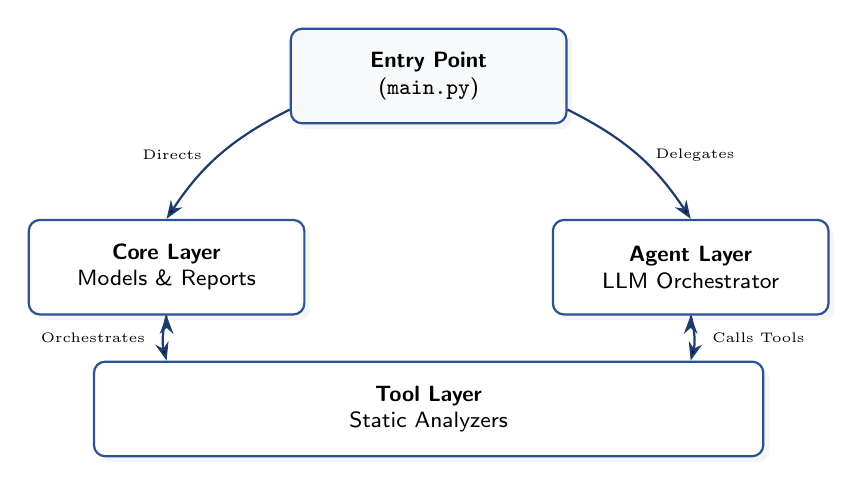
\begin{tikzpicture}[
        node distance=0.8cm and 2cm,
        layer/.style={draw=secondary, thick, rounded corners, fill=white, minimum width=3.5cm, minimum height=1.2cm, align=center, font=\sffamily\footnotesize, drop shadow={opacity=0.08}},
        arrow/.style={thick, ->, >=Stealth, draw=primary}
    ]
        \node[layer, fill=lightbg] (entry) {\textbf{Entry Point} \\ (\texttt{main.py})};
        \node[layer, below left=1.2cm and -0.2cm of entry] (core) {\textbf{Core Layer} \\ Models \& Reports};
        \node[layer, below right=1.2cm and -0.2cm of entry] (agent) {\textbf{Agent Layer} \\ LLM Orchestrator};
        \node[layer, below=3cm of entry, minimum width=8.5cm] (tools) {\textbf{Tool Layer} \\ Static Analyzers};

        \draw[arrow] (entry) edge[bend right=15] node[left, font=\tiny, xshift=-0.1cm] {Directs} (core.north);
        \draw[arrow] (entry) edge[bend left=15] node[right, font=\tiny, xshift=0.1cm] {Delegates} (agent.north);
        \draw[arrow] (core.south) edge[bend right=15] node[left, font=\tiny, xshift=-0.1cm] {Orchestrates} (tools.north -| core.south);
        \draw[arrow] (agent.south) edge[bend left=15] node[right, font=\tiny, xshift=0.1cm] {Calls Tools} (tools.north -| agent.south);
    \end{tikzpicture}
\end{frame}

\begin{frame}{Static Analyzers (Tool Layer)}
    The system delegates specialized tasks to five distinct, stateless tools:
    \vspace{1em}
    
    \begin{table}
        \centering
        \renewcommand{\arraystretch}{1.4}
        \begin{tabular}{p{3cm} p{10.5cm}}
            \toprule
            \textbf{\color{primary}Analyzer} & \textbf{\color{primary}Function} \\
            \midrule
            \textbf{Obfuscation} & Checks entropy, packing markers, and auto-unpacks (e.g. UPX). \\
            \textbf{Metadata} & Extracts format (PE/ELF), headers, sizes, and hashes. \\
            \textbf{Crypto} & Identifies cryptographic constants \& high-entropy blobs. \\
            \textbf{Strings} & Extracts and flags suspicious URLs, IPs, \& file paths. \\
            \textbf{Syscalls} & Maps imported APIs to MITRE ATT\&CK techniques. \\
            \bottomrule
        \end{tabular}
    \end{table}
\end{frame}

\begin{frame}{Agentic Orchestration}
    \textbf{LLM Integration (Agno + Gemini Flash Lite)}
    \vspace{1em}
    
    \begin{itemize}
        \item \textbf{Type-Safe Wrappers:} Python tools are exposed cleanly to the agent, eliminating signature mismatch issues.
        \item \textbf{Strict Constraints:} Prompts strictly forbid hallucinatory findings; assertions must map to real tool outputs.
        \item \textbf{Narrative Synthesis:} Provides analysts with an immediate, readable verdict instead of sifting through raw JSON dumps.
    \end{itemize}
\end{frame}

\begin{frame}{Evaluation \& Results}
    \textbf{Observed Findings (\texttt{fake\_malware} sample):}
    \vspace{1em}
    
    \begin{table}
        \centering
        \renewcommand{\arraystretch}{1.3}
        \begin{tabular}{lr | lr}
            \toprule
            \textbf{\color{primary}Metric} & \textbf{\color{primary}Value} & \textbf{\color{primary}Component Scores} & \textbf{\color{primary}Score} \\
            \midrule
            Risk Score & 36.0 / 100 & Strings & 100.0 \\
            Total Findings & 35 & Crypto & 45.0 \\
            Critical & 1 & Obfuscation & 35.0 \\
            High & 7 & Metadata & 0.0 \\
            Medium / Low & 19 / 8 & Syscalls & 0.0 \\
            \bottomrule
        \end{tabular}
    \end{table}
\end{frame}

\begin{frame}{Deployment \& Workflow}
    \begin{columns}[T]
        \column{0.45\textwidth}
        \textbf{\color{primary}Execution Modes}
        \vspace{0.5em}
        \begin{itemize}
            \item \texttt{--mode deterministic}
            \item \texttt{--mode agent}
            \item \texttt{--mode both}
        \end{itemize}
        
        \vspace{1em}
        \textbf{\color{primary}Auto-Unpacking}
        \vspace{0.5em}
        \begin{itemize}
            \item \texttt{--auto-unpack} \\ Re-evaluates packed payloads dynamically.
        \end{itemize}
        
        \column{0.45\textwidth}
        \textbf{\color{primary}Dockerized Runtime}
        \vspace{0.5em}
        \begin{itemize}
            \item Pre-packaged parsers (\texttt{pefile}, \texttt{pyelftools}).
            \item Pinned dependencies (UPX).
            \item Non-root secure execution.
            \item Simply execute: \\ \texttt{docker-compose run analysis}
        \end{itemize}
    \end{columns}
\end{frame}

\begin{frame}{Conclusion \& Future Work}
    \textbf{Conclusion}
    \begin{itemize}
        \item Successfully implemented an automated, dual-path triage system.
        \item Clean separation of parser logic, static heuristics, and LLM orchestration.
    \end{itemize}
    
    \vspace{1.5em}
    \textbf{Future Work}
    \begin{itemize}
        \item Agent integration with automatic unpacking (reusing artifacts).
        \item Save agent narrative output to persistent markdown artifacts.
        \item Introduce weighted risk scoring algorithms and deeper MITRE mappings.
    \end{itemize}
\end{frame}

\end{document}